\chapter{Fine-grained Cross Modal Retrieval}
\label{cha:Method}

In Chapter \ref{cha:scan} we explained in detail on the structure and principle behind our coarse-grained cross modal retrieval model. According to the result from running artworks datasets on the baseline model, there are aspects that we can focus on to make improvements. In this chapter, we will present our improved model of fine-grained cross modal retrieval.

The structure of this chapter is as follows. Section 4.1 gives a brief explanation on the processed artwork datasets and why these preprocessings are necessary for our model. Section 4.2 proposes our improved fine-grained cross modal retrieval model on fragment level instead of focusing on a whole image or sentence. Section 4.3 shows results of our presented model running on our annotated artworks datasets. Section 4.4 points out some existing shortcomings of our methodology and potential fields to be focused on in the future. Section 4.5 concludes this section.

\section{Dataset Preparation}
As we mentioned in Section \ref{cha:intro}, the datasets used in this thesis are from the Rijksmuseum Challenge by Mensink et al. \cite{MensinkICMIR2014}. The raw datasets were downloaded from the webpage dedicated to the Rijksmuseum Challenge. For each artwork, two files were available: a high resolution \verb|jpeg| image file and an accompanying \verb|xml| file including the metadata.

Python scripts (see Appendix \ref{app:A}) were written to parse the \verb|xml| files. Instead of using the raw captions, here the textual attributes we use are already processed into phrases. The technique here used is from Handler et al. \cite{nounphrase}, it extracts noun phrases from captions in raw \verb|xml| files which potentially helped us improve the accuracy as in most cases noun phrases contains more relevant information of artworks.  

As one single artwork can often have more than one annotation existed in its corresponding \verb|xml| file, it is important to extract all related annotations out and also combine them into one record for training and testing purpose, which saves computational power and simplifies the model input. 

According to captions and corresponding image labels, we can extract the corresponding image names. This extraction process is done using \verb|egyptian_convert.py| in Appendix \ref{app:A}, the captions for each image will have a corresponding \verb|txt| file created. For texting data, these \verb|txt| files are saved in \verb|phrase| directory and their corresponding image features in \verb|numpy| array format are saved under \verb|features| directory. Likewise, training phrases and image features are treated in the same way. These obtained \verb|txt| caption data will then be processed to extract noun phrases to achieve the retrieval in fragment level, results are saved in \verb|json| format. Our training and testing tasks will be based on these noun phrases and extracted image features.

\section{Fragment Retrieval}

\subsection{Overall Architecture}

\begin{figure}[h!]
\centering
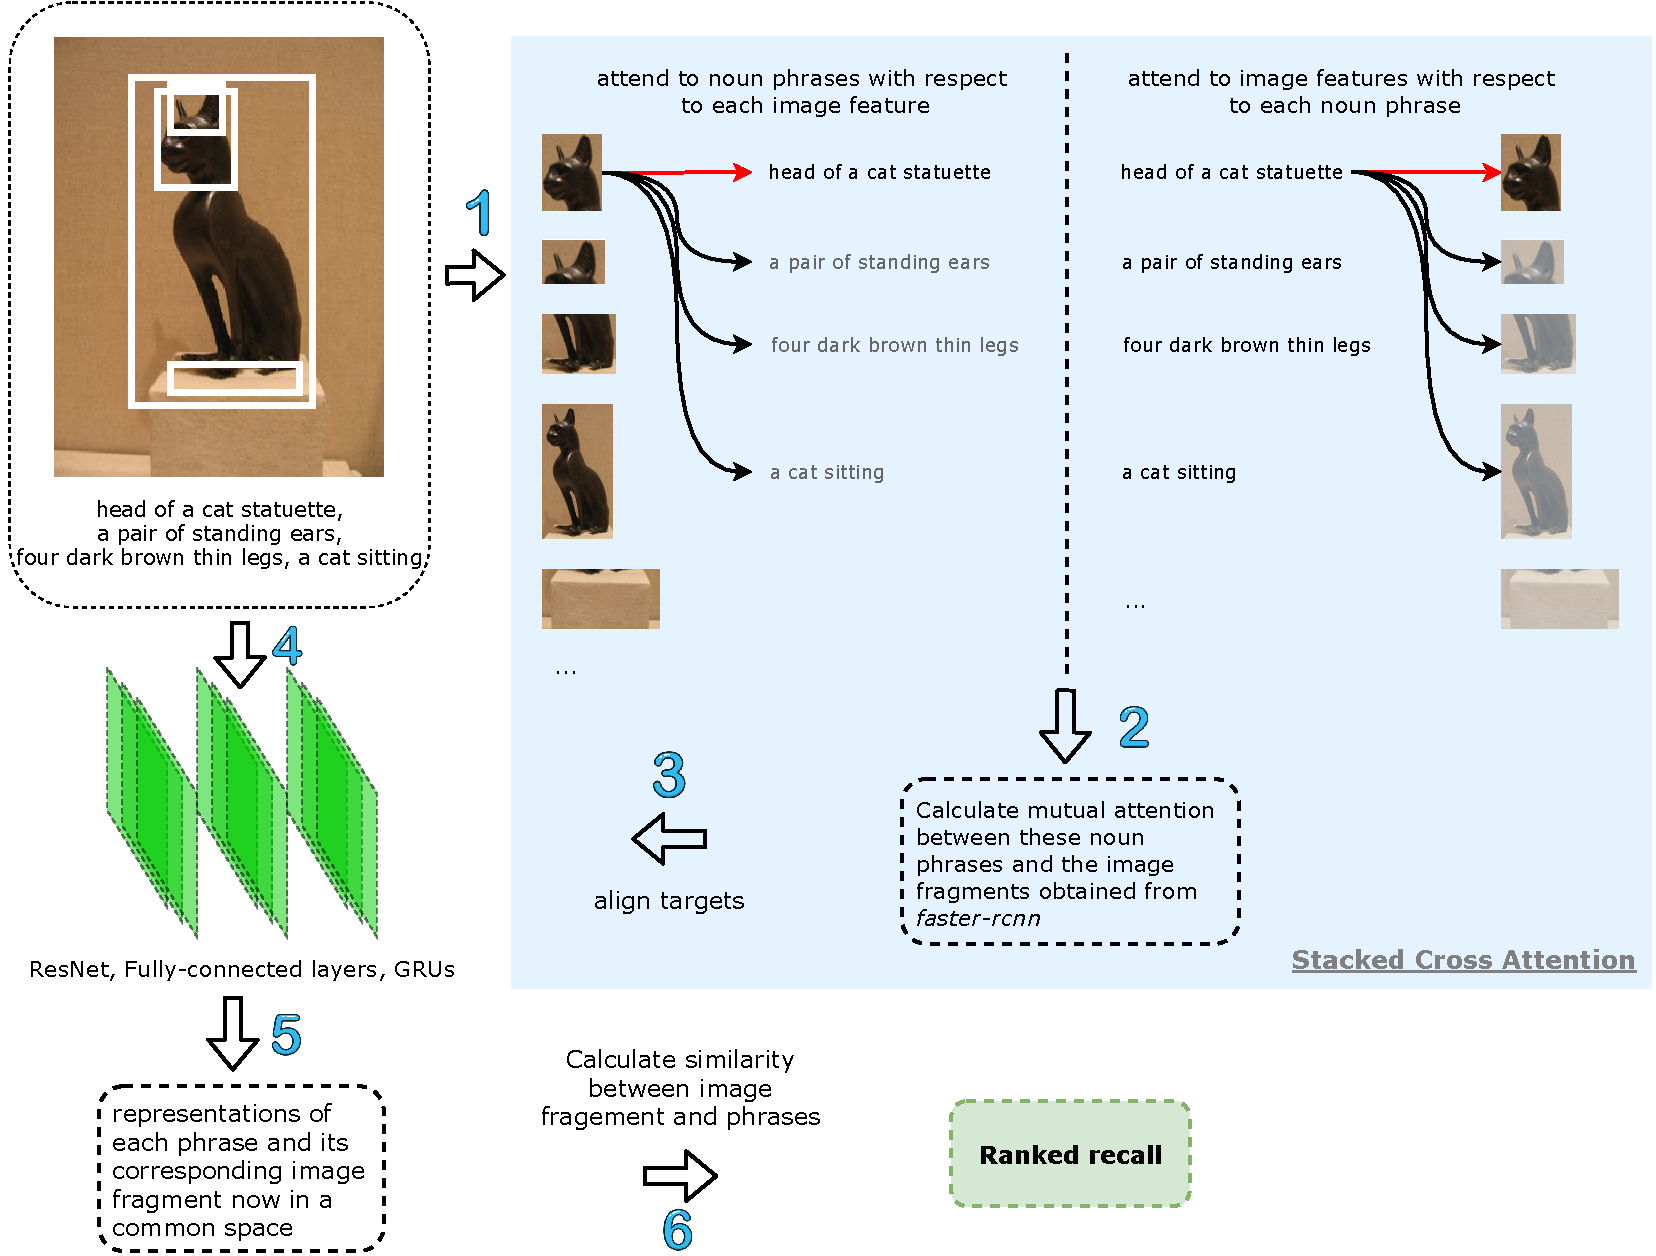
\includegraphics[width=\textwidth]{archi.pdf}
\caption{Fine-grained Cross Modal Retrieval Model Architecture}
\label{fig:mainarch}
\end{figure}


\section{Experiments}

\subsection{Ground Truth}

For this specific task, like we mentioned before, we used our manually annotated ground truth datasets. Each artwork has an updated \verb|xml| file which contains handcrafted image features and textural attributions. Here we show an example ground truth annotation in Figure \ref{fig:sampledata}.

\begin{figure}[h!]
\centering
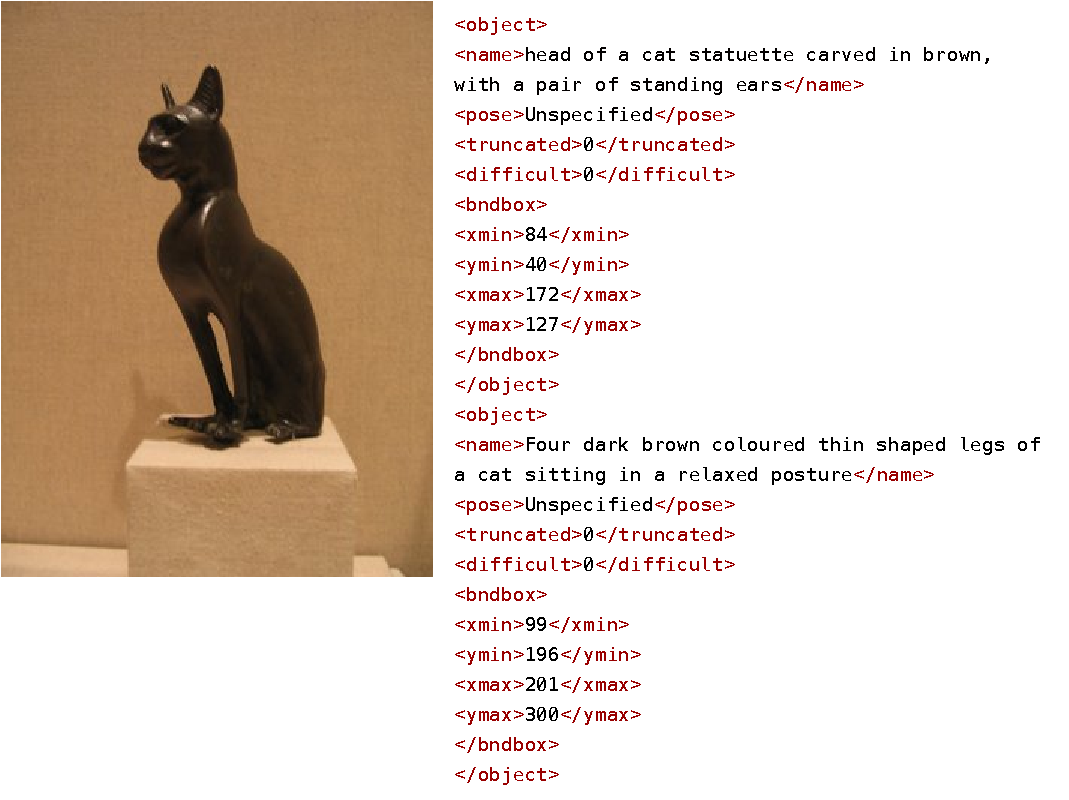
\includegraphics[width=0.6\textwidth]{sampledata.pdf}
\caption{Sample Artwork with Ground Truth Textual Attributes}
\label{fig:sampledata}
\end{figure}

From Figure \ref{fig:sampledata} we are look at an Egyptian artwork with a cat sculpture. For all object that exist in the artwork, those are, ``\textit{head of a	cat statuette carved in	brown, with	a pair of standing ears}'' and ``\textit{four dark brown coloured thin shaped legs of a cat sitting in a relaxed posture}'', each of them will have corresponding detailed location, pose, and truncated information attached. 

\subsection{Evaluation Metrics}

Recall is one of the most commonly used metric in the field of information retrieval. Here in this research project, we evaluate performance of sentence retrieval (image query) and image retrieval (sentence query) by recall at $K$ ($R@K$). This is defined as the fraction of queries for which the correct item is retrieved in the closest $K$ points to the query. Details of training and the bottom-up attention implementation are explained in Appendix \ref{app:n}.

\subsection{Results}

\section{Future Works}
Besides focusing on the fragment level image/sentence retrieval, it would also be beneficial to consider adopting a new image representation. 

Recently, some works \cite{TranslatingArtworks,parttowhole,Art2Real} have proposed new frameworks for artwork feature extraction and made prominent progress in the field. 


\section{Conclusion}


%%% Local Variables: 
%%% mode: latex
%%% TeX-master: "thesis"
%%% End: 
